\chapter{Application} \label{chap:application}

\section{Objectives}

Considering the GLLAMM model developed in previous chapters, its application on a real data set had a four-fold purpose:

\begin{enumerate}
	%
	\item \textbf{Evaluate the performance of the parametrizations.} We assessed if changing the posterior sampling geometry benefited the performance of the MCMC method.
	%
	\item \textbf{Assess psychometric properties.} We had a special interest in determine how difficult the items were, and in what part of the abilities measurement range they were located.
	%
	\item \textbf{Assess explanatory power of covariates.} We were interested on making hypothesis about the explanatory power a set of covariates had on the latent dimensions. 
	%
	\item \textbf{Evaluate the retrodictive accuracy.} We wanted to assess how well the model retrodicted the data, what was the evidence in favor of the proposed models, and what the model can tell to the educational authorities.
	%
\end{enumerate}

%%%%%%%%%%%%%%%%%%%%%%%%%%%%%%%%%%%%%%%%%%%%%%%%%%%%%%%%%%%%%%%%%%%%%%%

\section{Instrument}

The evaluation instrument was selected from the Peruvian public teaching career national assessment. The large standardized test took place during $2017$, an it allowed the winner to obtain an appointment, or temporal hiring, into the public teaching career of Peru. 

The instrument was composed of $90$ multiple-choice question, with four alternatives per item. The items were scored on a dichotomous scale, that is, only one of the four alternatives was the correct one. Moreover, the test was organized in three sub-tests designed to evaluate the reading comprehension, mathematical reasoning, and pedagogical knowledge of the applicants. Given the extension and differences between the sub-tests, we decided to focus on the reading comprehension portion, composed of the first $25$ items of the instrument. 

The reading comprehension sub-test was designed to evaluate the teacher's ability to reconstruct the meaning of different types of texts, presented in diverse formats. The sub-test had items designed to measure only one of the three hierarchically nested sub-dimensions of reading comprehension: literal, inferential, and reflective abilities. The literal ability items centered its focus on assessing the teacher's capability to locate explicit information on the texts. The inferential items assessed the teacher's ability to integrate the information in texts, with the goal of inferring its theme, purpose or implicit logic relationships. Lastly, the reflective items evaluated the teacher's abilities to critically reflect about the content and structure of texts.

Finally, besides being nested in dimensions, the items were bundled in groups of five, to a common text or passage, that provided the stimulus over which the individual was assessed, i.e. the items were testlets. 


%%%%%%%%%%%%%%%%%%%%%%%%%%%%%%%%%%%%%%%%%%%%%%%%%%%%%%%%%%%%%%%%%%%%%%%
%%%%%%%%%%%%%%%%%%%%%%%%%%%%%%%%%%%%%%%%%%%%%%%%%%%%%%%%%%%%%%%%%%%%%%%

\section{Data}

The access to data set was done through the proper legal requirement of open information to the Ministry of Education of Peru (MINEDU). The data set was anonymized and transferred through digital mean to the researcher.

Finally, given the large amount of individuals exposed to the aforementioned evaluation, approximately $194,000$, a simple random sample of $2,000$ individuals was taken.

%%%%%%%%%%%%%%%%%%%%%%%%%%%%%%%%%%%%%%%%%%%%%%%%%%%%%%%%%%%%%%%%%%%%%%%
%%%%%%%%%%%%%%%%%%%%%%%%%%%%%%%%%%%%%%%%%%%%%%%%%%%%%%%%%%%%%%%%%%%%%%%

\section{Results}

Figure \ref{fig:design} shows the path diagram of the hypothesized dimensional structure, for the hierarchical cross-classified IRT model corresponding with the instrument. The figure represents the responses of one person on $12$ items.
%
\begin{figure}[H]
	\centering
	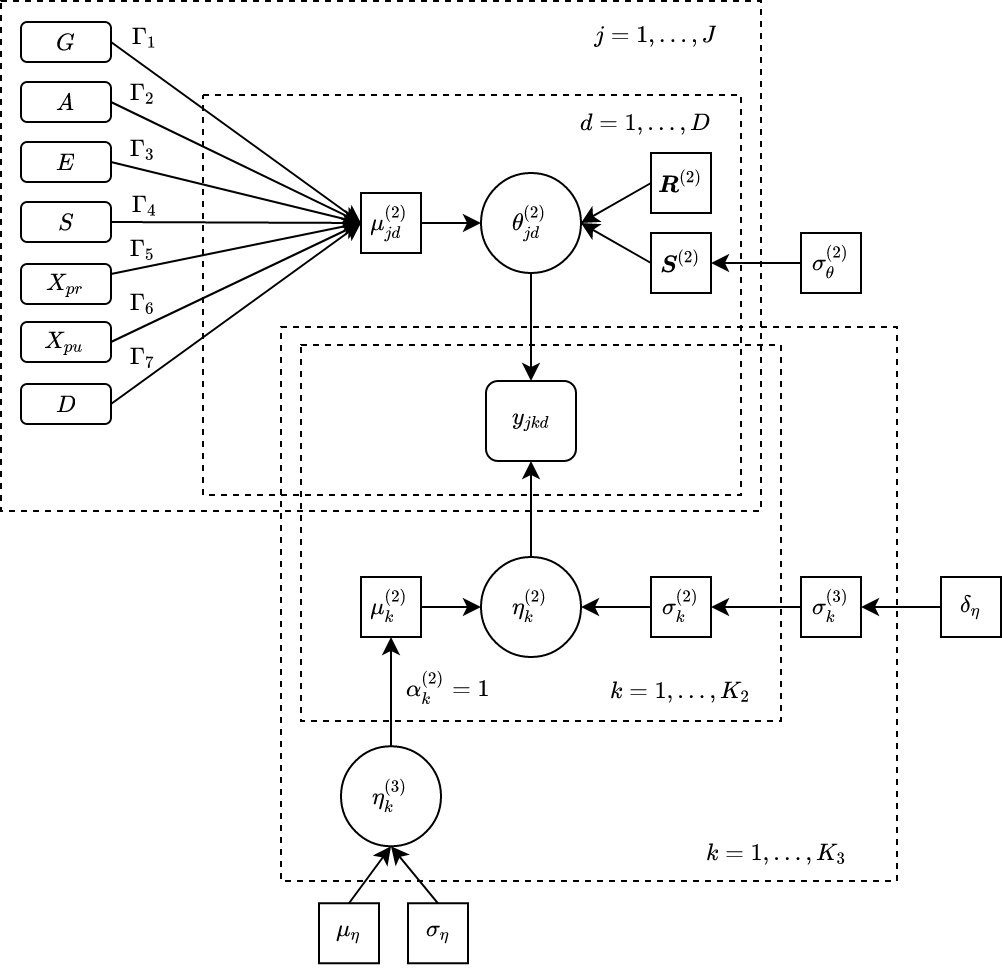
\includegraphics[width=0.8\linewidth]{app_FOLV_dag}
	%
	\caption[Directed Acyclic Graph (DAG). Application's first-order latent variable model (FOLV).]%
	{Directed Acyclig Graph (DAG). Application's first-order latent variable model (FOLV). Circles represent latent variables. Squares represent parameters or parameters for priors. Large squares represent nesting in specific units.}
	\label{fig:FOLV_app}
\end{figure}
%
\begin{figure}[H]
	\centering
	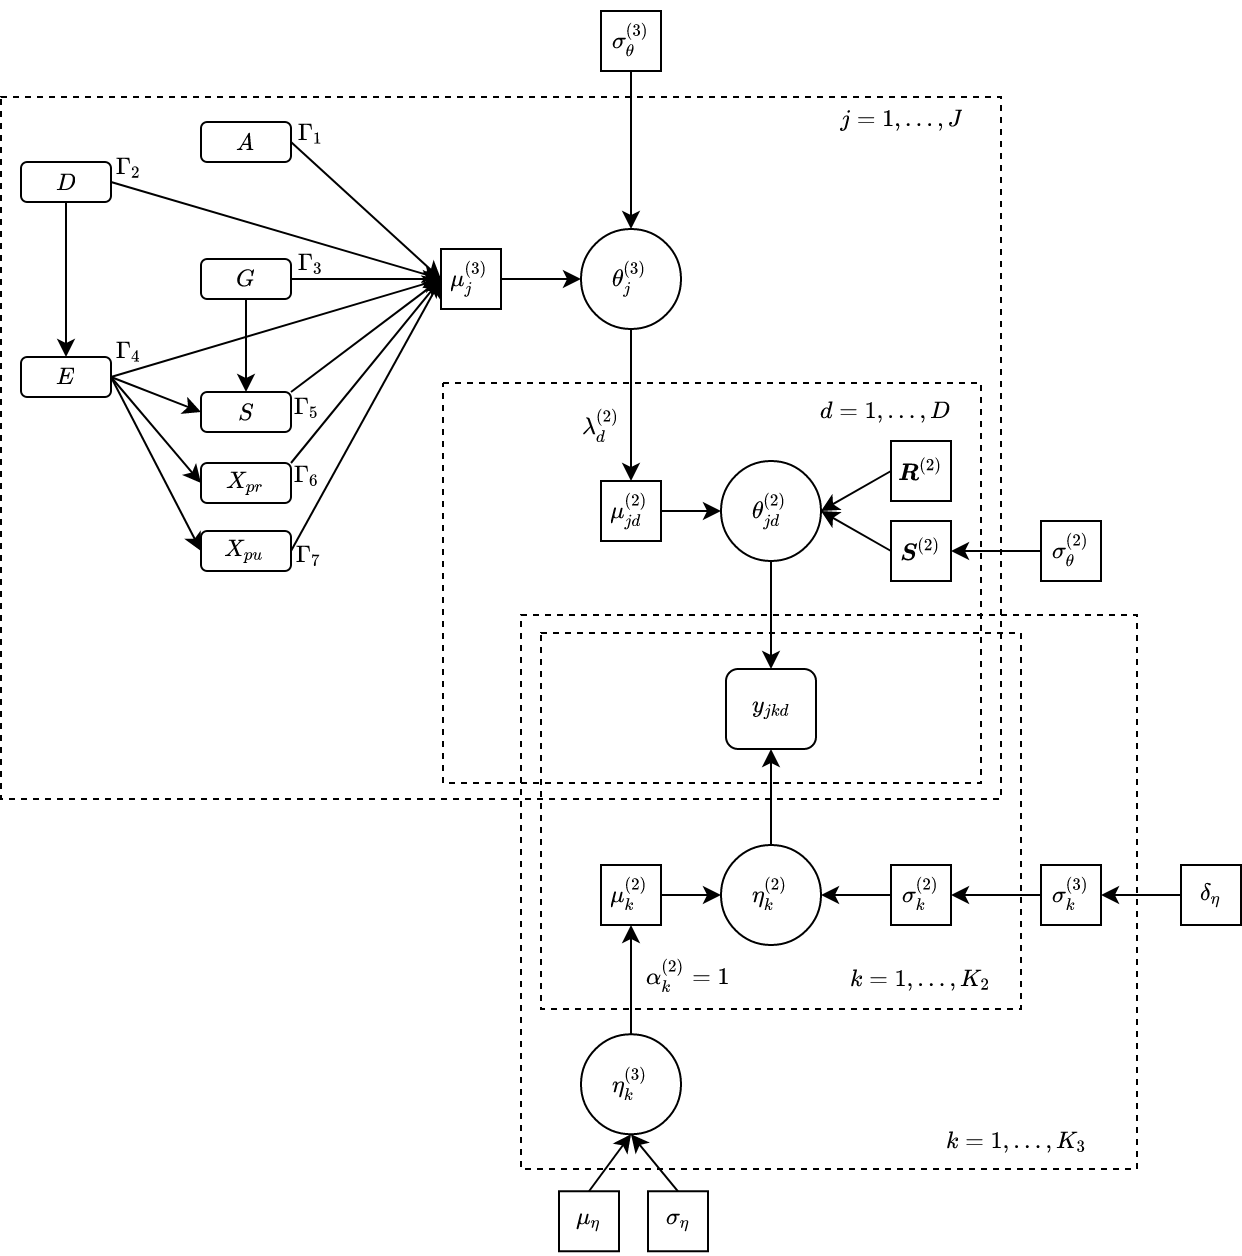
\includegraphics[width=0.8\linewidth]{app_SOLV_dag}
	%
	\caption[Directed Acyclic Graph (DAG). Application's second-order latent variable model (SOLV).]%
	{Directed Acyclig Graph (DAG). Application's second-order latent variable model (SOLV). Circles represent latent variables. Squares represent parameters or parameters for priors. Large squares represent nesting in specific units.}
	\label{fig:SOLV_app}
\end{figure}

%%%%%%%%%%%%%%%%%%%%%%%%%%%%%%%%%%%%%%%%%%%%%%%%%%%%%%%%%%%%%%%%%%%%%%%

\subsection{Parametrization performance}

%
\begin{figure}[H]
	\centering
	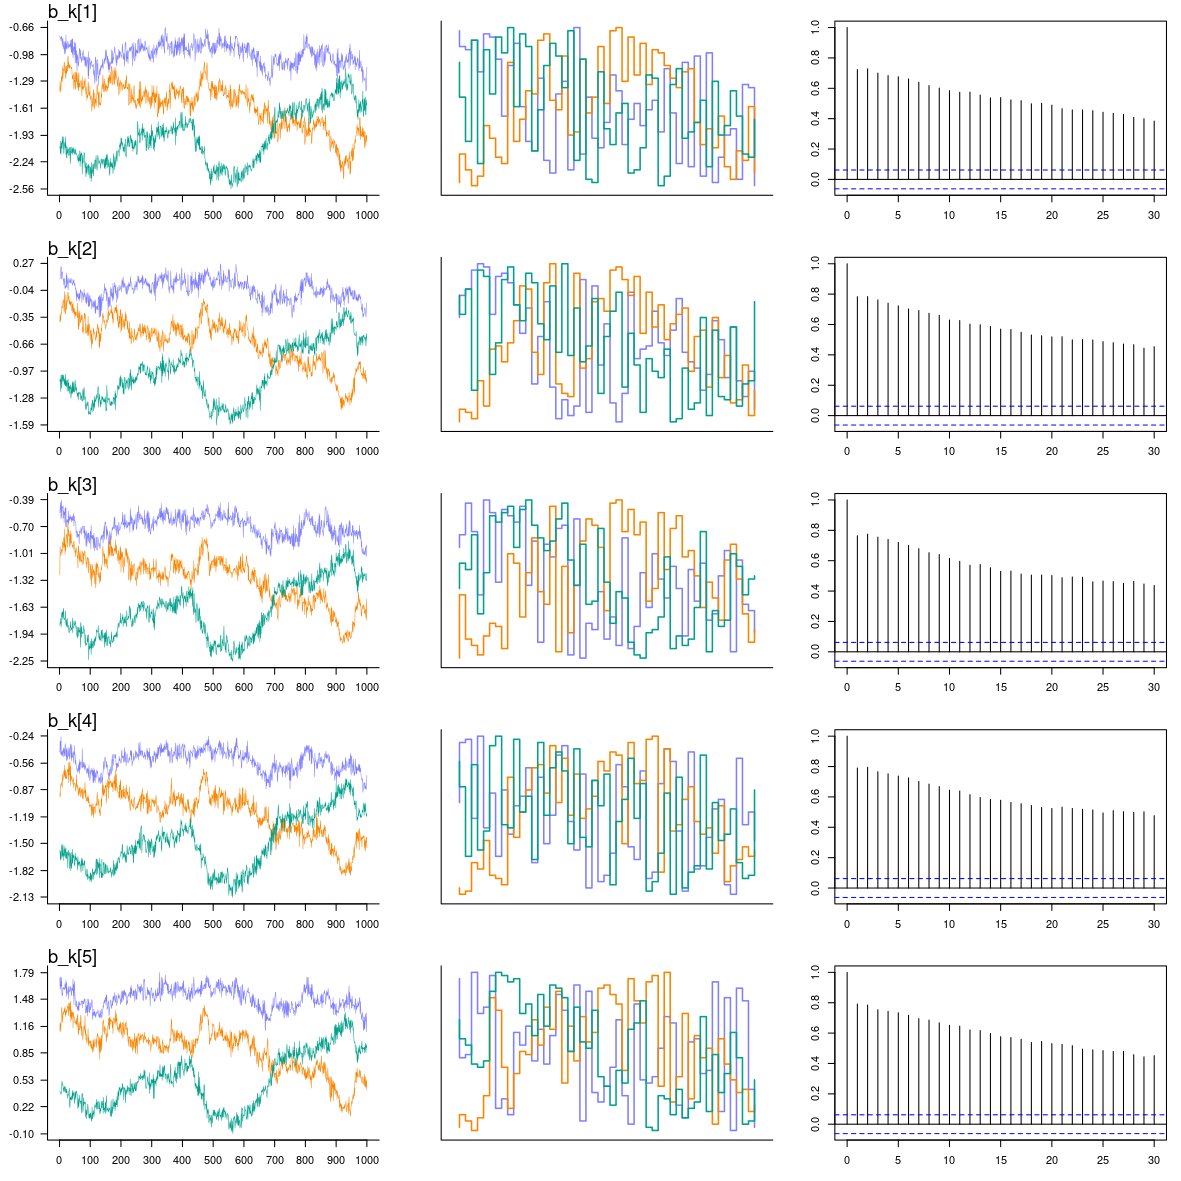
\includegraphics[width=1\linewidth]{FOLV_CE_bk_1_5}
	%
	\caption[Application's first-order latent variable model (FOLV). Centered parametrization. Items difficulty. Trace, trank and auto-correlation plots.]%
	{Application's first-order latent variable model (FOLV). Centered parametrization. Items difficulty: (Left) trace plot, (Middle) trank plot, (Right) auto-correlation plot.}
	\label{fig:FOLV_CE_chains1}
\end{figure}
%
\begin{figure}[H]
	\centering
	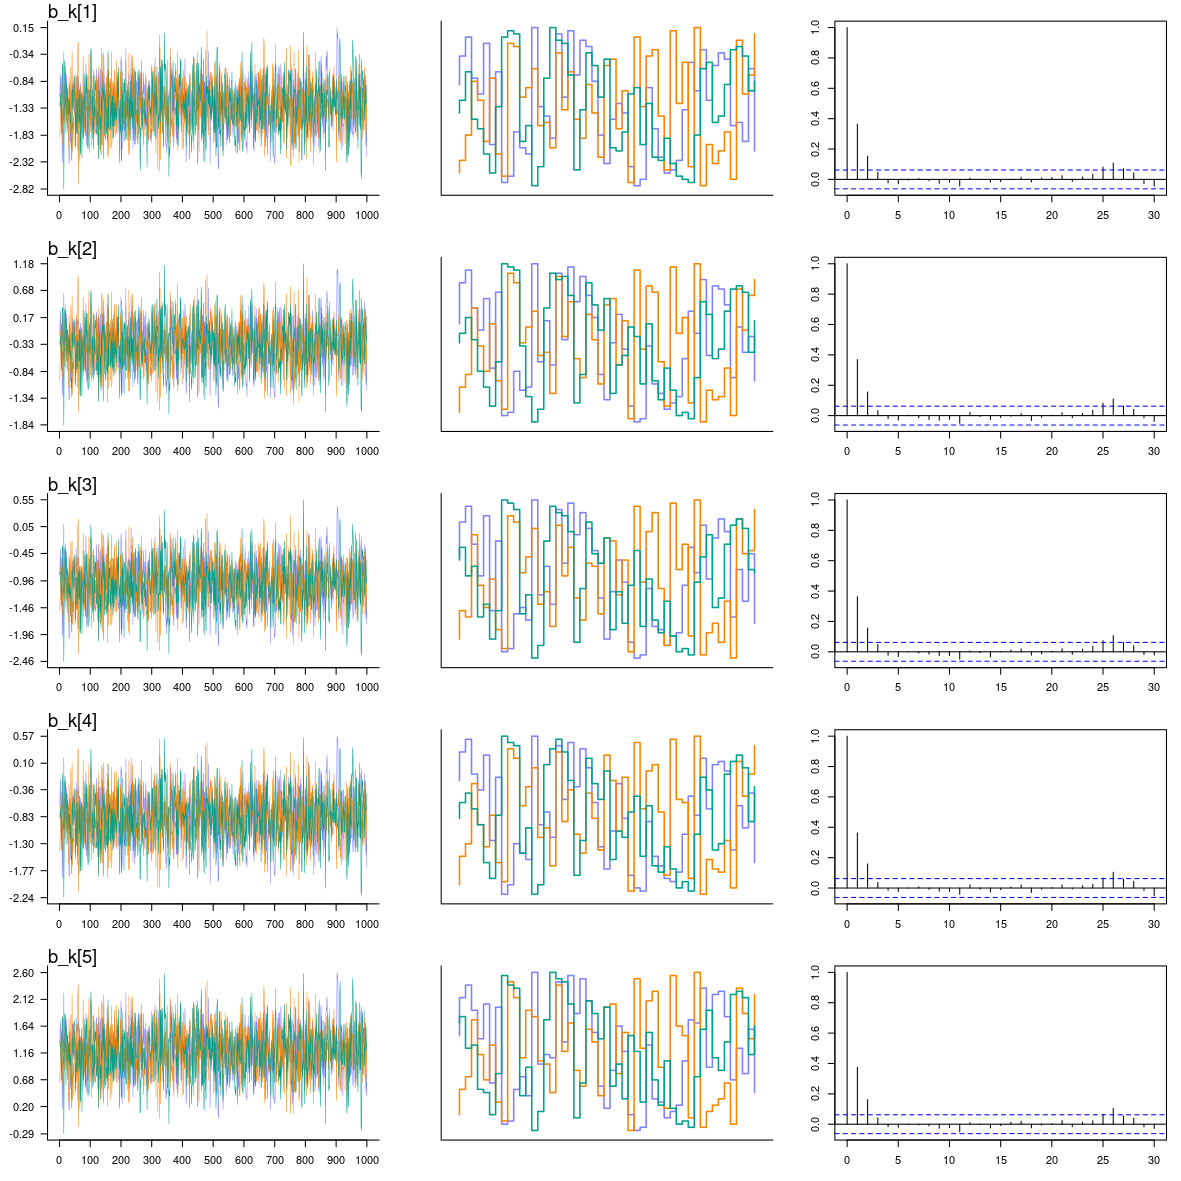
\includegraphics[width=1\linewidth]{FOLV_NC_bk_1_5}
	%
	\caption[Application's first-order latent variable model (FOLV). Non-centered parametrization. Items difficulty. Trace, trank and auto-correlation plots.]%
	{Application's first-Order latent variable model (FOLV). Non-centered parametrization. Items difficulty: (Left) trace plot, (Middle) trank plot, (Right) auto-correlation plot.}
	\label{fig:FOLV_NC_chains1}
\end{figure}
%
\begin{figure}[H]
	\centering
	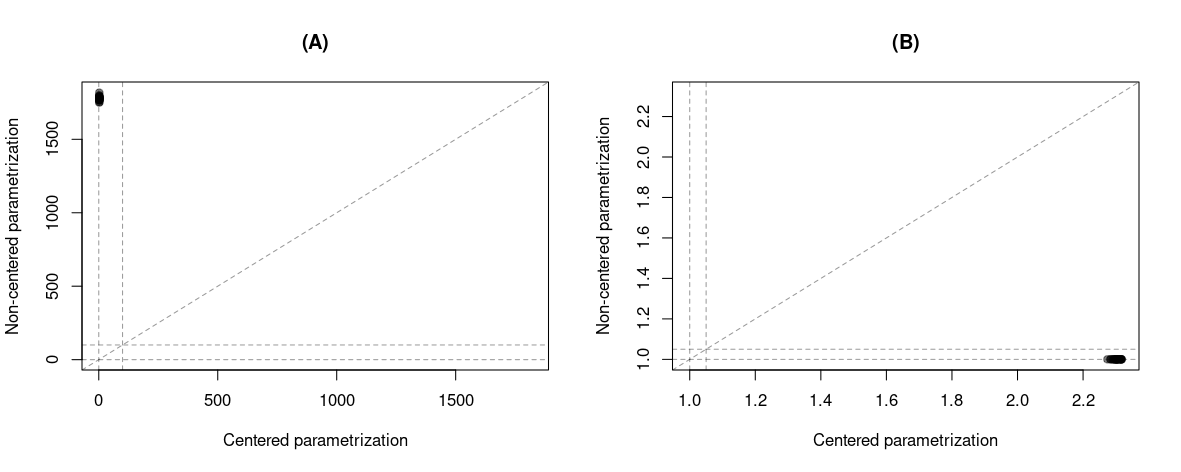
\includegraphics[width=1\linewidth]{FOLV_stat_bk}
	%
	\caption[Application's first-order latent variable model (FOLV). CP and NCP comparison plot.]%
	{Application's first-order latent variable model (FOLV). CP and NCP comparison plot. (A) \texttt{n\_eff} for items' difficulties. (B) \texttt{Rhat} for items' difficulties. Diagonal discontinuous line describes equality between CP and NCP. Vertical and horizontal discontinuous lines set in A corresponds to \texttt{n\_eff}$=100$. Vertical and horizontal discontinuous lines set in B corresponds to \texttt{Rhat}$=1.05$. }
	\label{fig:FOLV_stat1}
\end{figure}


%%%%%%%%%%%%%%%%%%%%%%%%%%%%%%%%%%%%%%%%%%%%%%%%%%%%%%%%%%%%%%%%%%%%%%%

\subsection{Psychometric properties}

As in any standardized evaluation, instrument developers have a special interest in determine how difficult the items were, and in what part of the abilities measurement range they were located.

of were wants to assess  Pychometric properties of the items and texts, texts is an extra
%
\begin{figure}[H]
	\centering
	\begin{subfigure}
		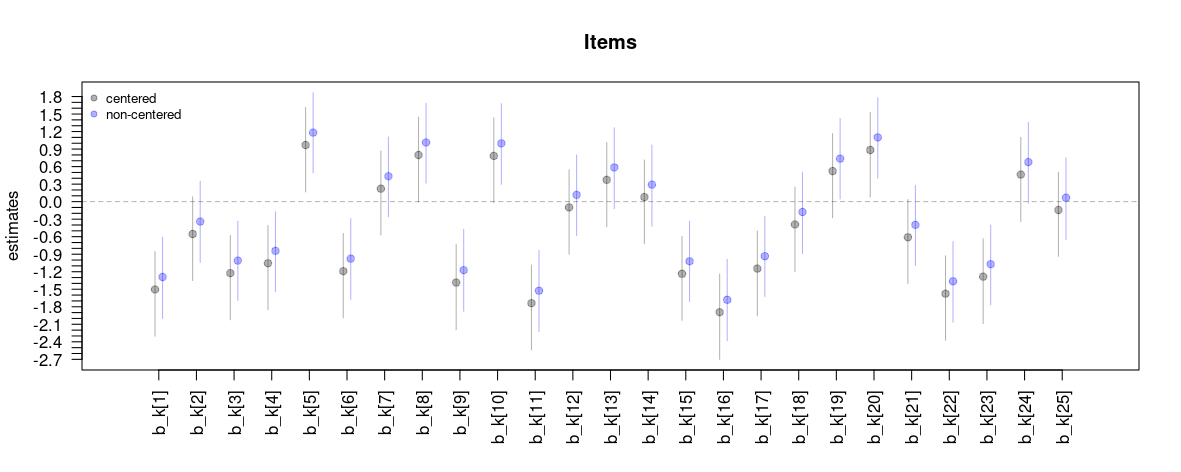
\includegraphics[width=0.9\linewidth]{FOLV_recovery_items}
	\end{subfigure}
	%
	\begin{subfigure}
		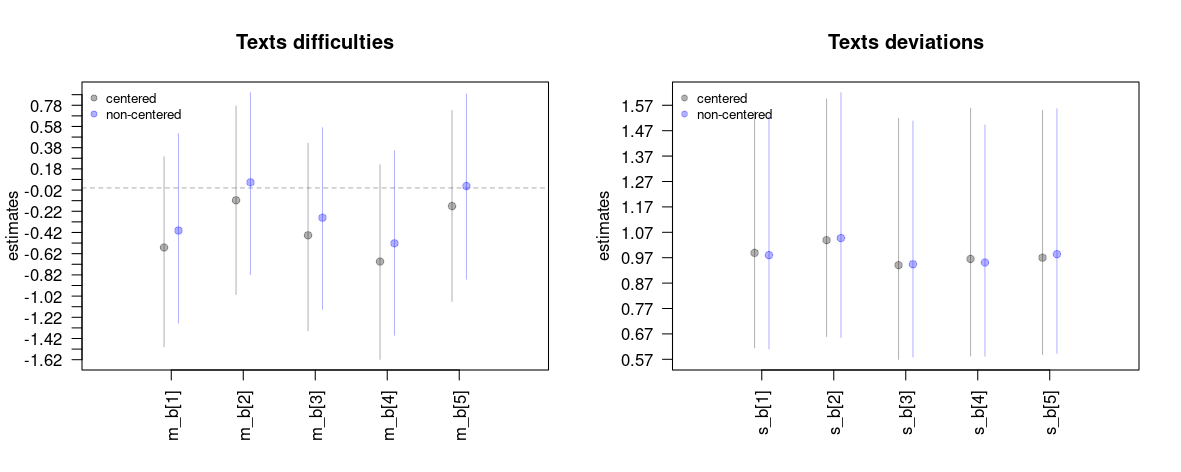
\includegraphics[width=0.87\linewidth]{FOLV_recovery_texts}
	\end{subfigure}
	%
	\caption[Application's first-order latent variable model (FOLV). Centered and non-centered parametrization. Items, and texts difficulties, and texts deviations.]%
	{Application's first-order latent variable model (FOLV). Centered and non-centered parametrization. Items, and texts difficulties, and texts deviations.}
	\label{fig:FOLV_CE.NC_recovery}
\end{figure}


%%%%%%%%%%%%%%%%%%%%%%%%%%%%%%%%%%%%%%%%%%%%%%%%%%%%%%%%%%%%%%%%%%%%%%%

\subsection{Explanatory power}

%
\begin{figure}[H]
	\centering
	\begin{subfigure}
		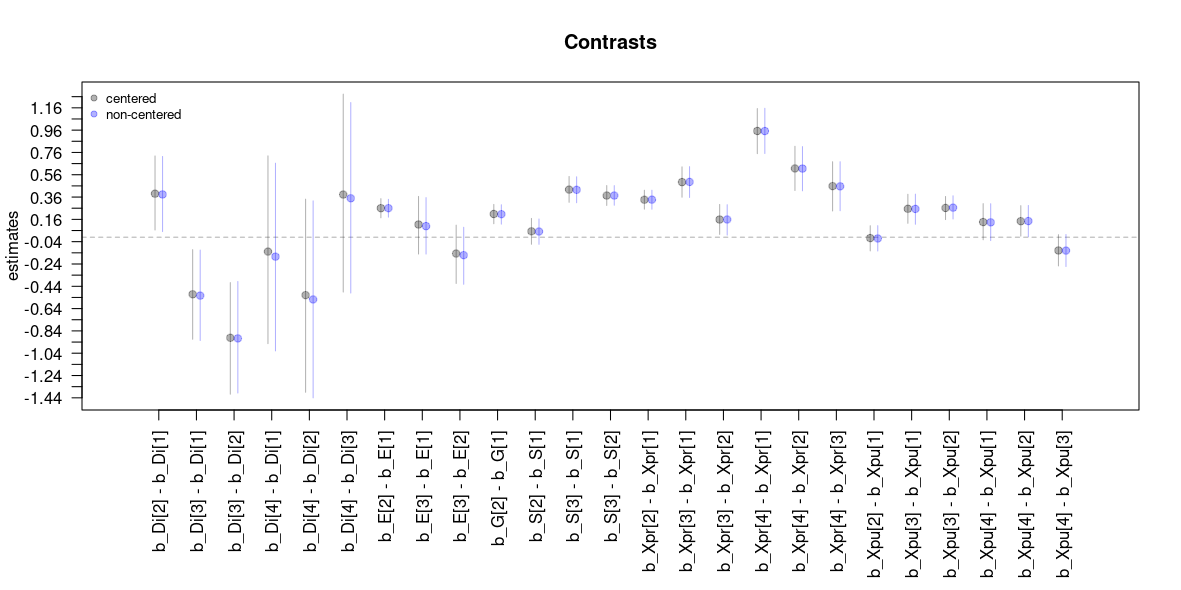
\includegraphics[width=0.9\linewidth]{FOLV_recovery_contrast}
	\end{subfigure}
	%
	\begin{subfigure}
		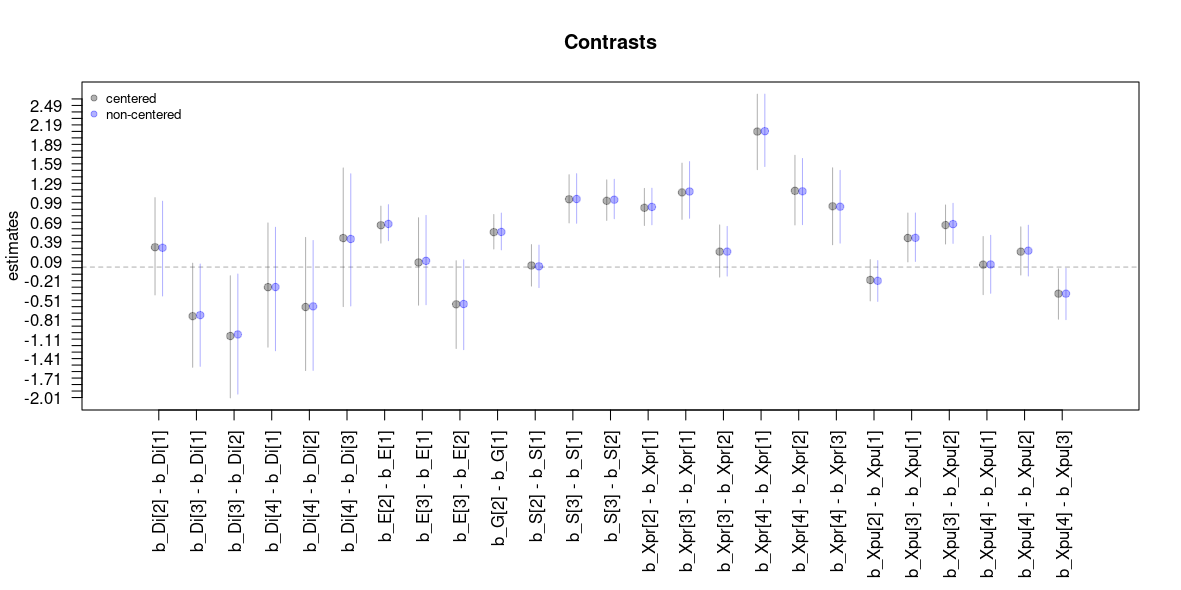
\includegraphics[width=0.9\linewidth]{SOLV_recovery_contrast}
	\end{subfigure}
%
	\caption[Application's first- and second-order latent variable model. CP and NCP comparison plot.]%
	{Application's first- and second-order latent variable model. CP and NCP comparison plot. (Top panel) Contrasts in the FOLV model. (Bottom panel) Contrasts in the SOLV model. }
	\label{fig:contrast_both}
\end{figure}

%%%%%%%%%%%%%%%%%%%%%%%%%%%%%%%%%%%%%%%%%%%%%%%%%%%%%%%%%%%%%%%%%%%%%%%

\subsection{Retrodictive accuracy}

Pareto-smoothed importance sampling cross-validation (PSIS) and the  Widely Applicable Information Criterion (WAIC).

All of the preceding suggests one way to navigate overfitting and underfitting: Evaluate our models out-of-sample. using cross validation and information criteria


with an additional set of :covariates (not used in the model), we examine their classification and access to the pubic teaching career. 

how the classified poeple is characterized, math scales vs the scores (cut-of of 30 points, or 15 items, 2 points / item)

characterize individuals into profiles 




